%
% main.tex -- Paper zum Thema "Extreme Ereignisse"
%
% (c) 2018 Melina Staub, Hochschule Rapperswil
%
\chapter{Extreme Ereignisse\label{chapter:thema}}
\lhead{Extreme Ereignisse}
\begin{refsection}
\chapterauthor{Melina Staub}


\section{Einleitung}
Fast täglich erscheinen Schlagzeiten wie diese in der Zeitung:

\begin{itemize}
\item Wetter-Extreme häufen sich auch in der Schweiz
\item Seit Lothar wird es der vielleicht stärkste Sturm
\item Die Schweiz reagiert empfindlich auf Wetteränderung
\item Unwetter sorgten für eine chaotische Nacht
\item Schweiz besonders stark vom Klimawandel betroffen
\end{itemize}

Doch wieviel Wahrheit steckt in diesen Headlines? Sind sie nur Hirngespinste der Nachrichtenindustrie? Wollen uns die Medien täuschen oder geht da draussen wirklich etwas vor sich?

Dass die Natur im Wandel ist, steht ausser Frage. In der Geschichte der Erde waren extreme Ereignisse keine Seltenheit. Ob Eiszeiten, Trockenperioden oder lang anhaltende Regenschauer, wohl jedes vorstellbare Ereignis ist vorgekommen. Vulkanausbrüche pumpten Kohlendioxid in die Atmosphäre und Meteoriteneinschläge lösten Tsunamis aus, welche die Landflächen fluteten. Die Erde hat sich von Zeit zu Zeit und nach jedem Ereignis erholt oder angepasst. Doch seit Mitte des 18. Jahrhunderts und somit mit der Industrialisierung hat sich viel verändert.

Die nachfolgenden Seiten wurden ohne Vorurteile oder frühzeitigen Feststellungen rund um den Klimawandel erstellt. Am Ende soll die Wahrheit festgestellt werden.
Was bereits klar ist, die Erde wird den Klimawandel überstehen, wie sie auch schon extreme Trockenperioden oder Eiszeiten überlebt hat. Doch was wird mit uns?


\section{Was sind extreme Ereignisse?}
Die Diskussionen um den Klimawandel erregt die Gemüter auf der ganzen Welt. Einige verleugnen ihn und andere verstehen ihn und tun alles um ihn zu stoppen. Besonders extreme Ereignisse wie starke Regenfälle und die daraus resultierenden Überschwemmungen und Verwüstungen bleiben uns stark in Erinnerung.
Eben diese Ereignisse weichen stark von den Durchschnittswerten ab und hinterlassen oft grosse Schäden und ebenso grosse Schadensummen. Doch nicht nur überdurchschnittlich starke Ereignisse, sondern auch sehr kleine wie Trockenperioden oder Wasserknappheit sind extreme Ereignisse.
Jetzt stellt sich die Frage, ob diese extremen Ereignisse natürlichen Ursprungs sind, also  die Anordnung durch den Zufall bestimmt wird und auch ohne den Einfluss des Menschen passiert wären oder ob diese auf den Klimawandel zurückzuführen sind und somit eine unnatürliche Häufung aufzeigen.


\subsection{Aufzeichnungen in der Schweiz}
In den \textit{Schweizer Wetterjahresbücher} und \textit{Analen der Schweizerischen Meteorologischen Zentralanstalt} lassen sich Wetter- und Klimadaten bis ins Jahr 1864 abrufen. Umfangreiche Tabellen und Berichte sind für Wetter- und Klimainteressierte ein historisch sehr bedeutender Datenschatz. 
Der Monatliche Wetterverlauf wurde ab dem Jahr 1911 geführt, extreme Wetterereignisse in Berichten beschrieben und aufgezeichnet (Abbildung \ref{Analen}). Die Analen wurden 2011 durch den Klimareport abgelöst. Seit dem Jahr 2011 sind der Klimabericht wie auch die Analen für die Öffentlichkeit zugänglich und können Online eingesehen werden.
Mit diesen langen und genauen Klimadaten lässt sich tief in die Vergangenheit des Schweizer Klima blicken. Ein Blick in die Klima-Vergangenheit wird möglich.

\begin{figure}
\centering
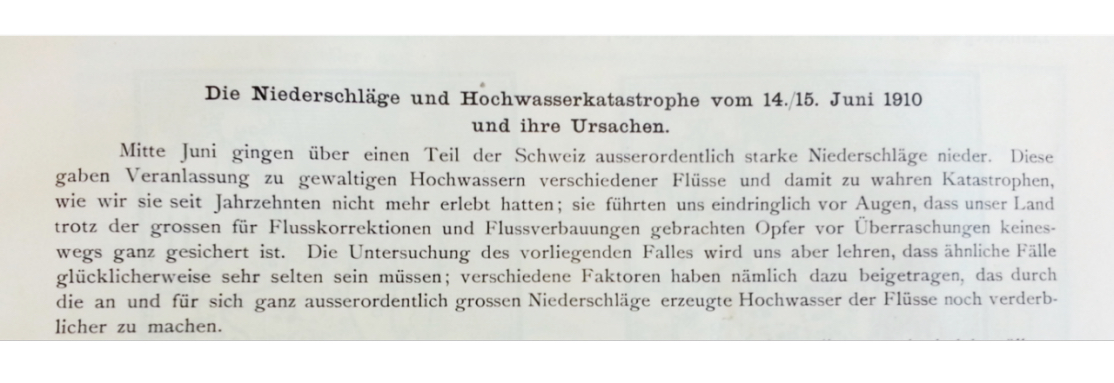
\includegraphics[width=\hsize]{extrem/Analen.jpg}
\caption{Originaltext aus den Annalen 1910 zur Hochwasserkathastrophe vom Juni 1910. (Quelle: MeteoSchweiz)}
\label{Analen}
\end{figure}


\subsection{Homogene Messreihen}
Um die Klimadaten der letzten 150 Jahren miteinander zu vergleichen, müssen die Messergebnisse vor dem Vergleich homogensisiert werden (Abbildung \ref{Homogen}). Die Modernisierung der Messgeräte,  eine Verschiebung des Messstandortes oder die Veränderung der Umgebung führen zu anderen Messwerten als beispielsweise diese des Vorgänger Messgeräts. Die Daten liefern einen verfälschten Vergleich, wenn man sie ohne Homogenisierung miteinander vergleicht.
Wenn man den Messstandort verlegt, verändert sich die Höhenlage. Dies wirkt sich auf die Temperaturmessung aus, da sich diese mit der Höhe im Mittel verschiebt. Die Messreihe wird ungenau und ein verfälschtes Bild zeichnet sich ab, welches nichts mit dem Klima zu tun hat.
Um diese Fehlinterpretationen zu vermeiden, sind in den \textit{Schweizer Wetterjahresbücher} und \textit{Analen der Schweizerischen Meteorologischen Zentralanstalt} sämtliche Messwerte homogenisiert worden. Ein direkter Vergleich wird so möglich.

\begin{figure}
\centering
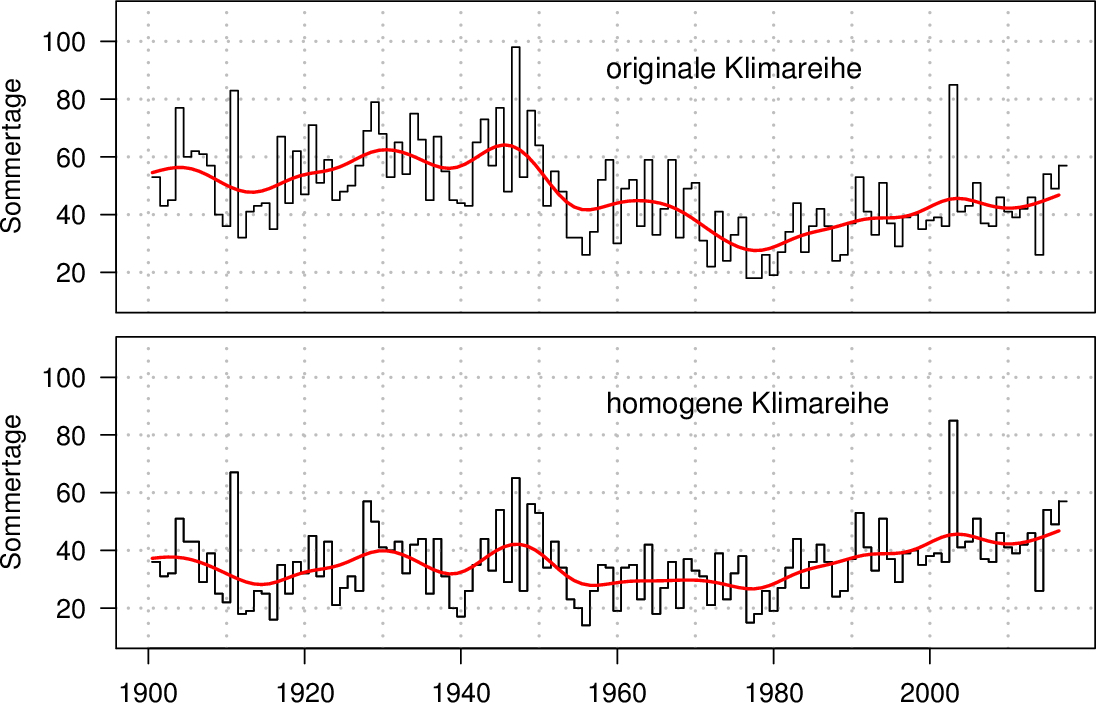
\includegraphics[width=0.6\textwidth]{extrem/Homogen.jpg}
\caption{Entwicklung der Anzahl Sommertage (Maximum--Temperatur $\ge 25^{\circ}$C ) pro Jahr an der Messstation Zürich/Fluntern seit 1901, gerechnet aus der originalen und homogenen Temperatur--Messreihe. Der geglättete Verlauf ist rot eingezeichnet. (Quelle: MeteoSchweiz)}
\label{Homogen}
\end{figure}


\section{Unwetterlotto}
Um herauszufinden ob extreme Ereignisse nicht durch den Zufall bestimmt werden, benötigen wir vorerst ein Modell um diese Berechnungen durchführen zu können.
Hierbei bedienen wir uns dem Glücksspiel, genauer gesagt dem Lotto.

\begin{figure}
\centering
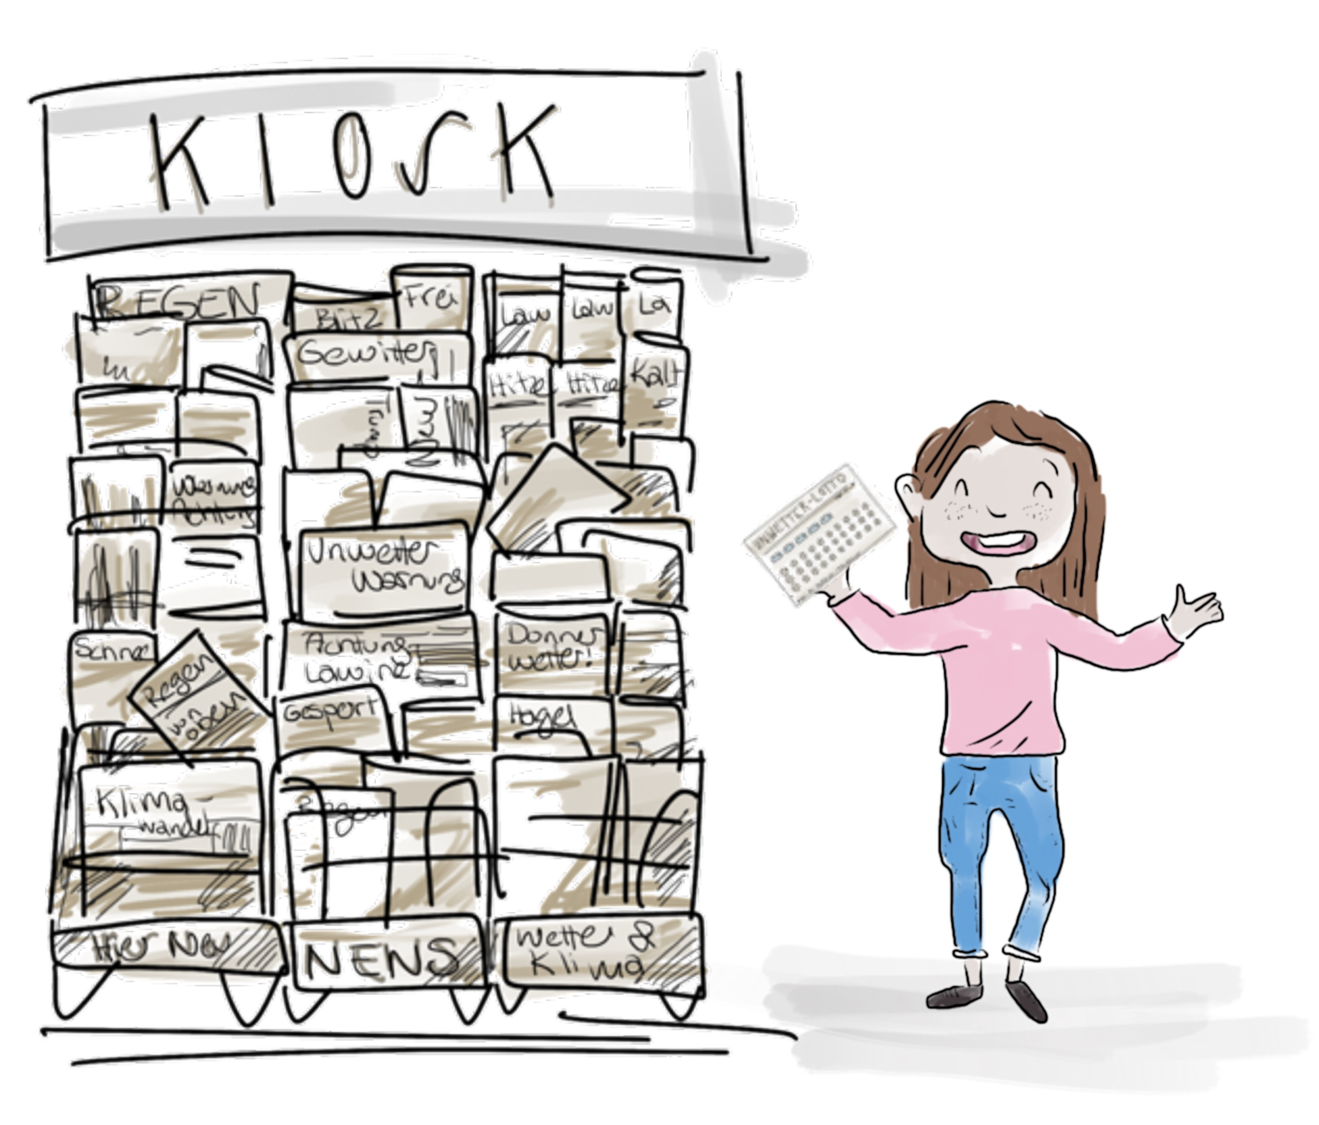
\includegraphics[width=0.4\textwidth]{extrem/Kiosk.pdf}
\caption{Unwetterlottoschein exklusiv erhältlich für Mathsem Teilnehmer.}
\label{Kiosk}
\end{figure}

Exklusiv für die Leserinnen und Leser dieses Seminarbuches steht der Unwetterlottoschein zur Verfügung, welchen man am Zeitungskiosk (Abbildung \ref{Kiosk}) erwerben und statt auf Zahlen auf Unwetterereignisse tippen kann. Auf dem Unwetter-Lotto-Schein (Abbildung \ref{Lottoschein}) kann wie beim normalen Zahlenlotto aus verschiedenen Zahlen ausgewählt und seine Tipps abgeben werden. Danach gibt es eine Unwetterziehung, welche mit den abgegebenen Tipps verglichen werden können.

\begin{figure}
\centering
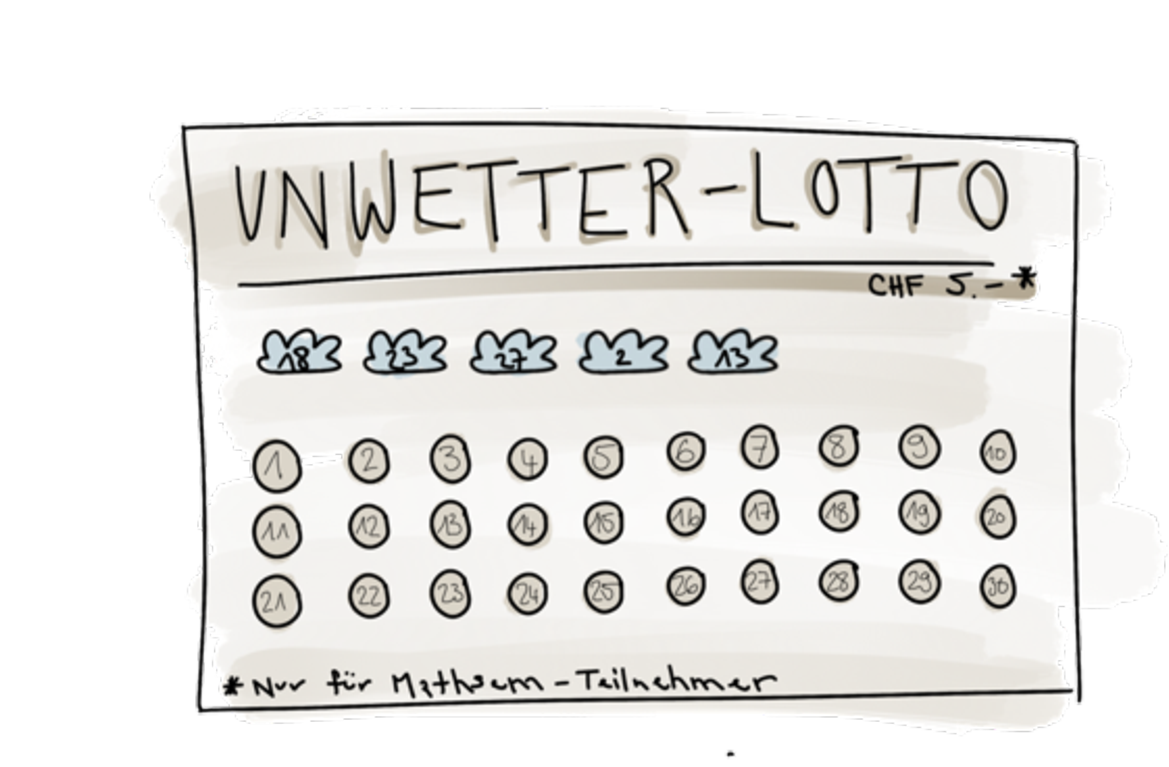
\includegraphics[width=0.7\textwidth]{extrem/Lottoschein.pdf}
\caption{Unwetterlottoschein.}
\label{Lottoschein}
\end{figure}

Die Kugeln 1-30 beschreiben alle vorhandenen Ereignisse, welche wir \textcolor{red}{\textbf{N}} nennen. Die fünf Wolken stehen für die Anzahl Kreuze, welche wir machen dürfen. Das heisst, welche Unwetter \textcolor{blue}{\textbf{n}} wir aus den totalen Ereignissen 1-30 auswählen dürfen. Die bei der Unwetterziehung gezogenen Ereignisse \textcolor{green}{\textbf{M}} sind unsere Stichproben aus allen Ereignissen.

Jetzt stellen wir uns die entscheidende Frage: 
Wie wahrscheinlich ist es, ein 5er im Unwetter-Lotto (Abbildung \ref{WahrscheinlichkeitUnwetterlotto})zu erhalten? Diese Wahrscheinlichkeit bezeichnen wir mit \textcolor{yellow}{\textbf{k}}.

\begin{figure}
\centering
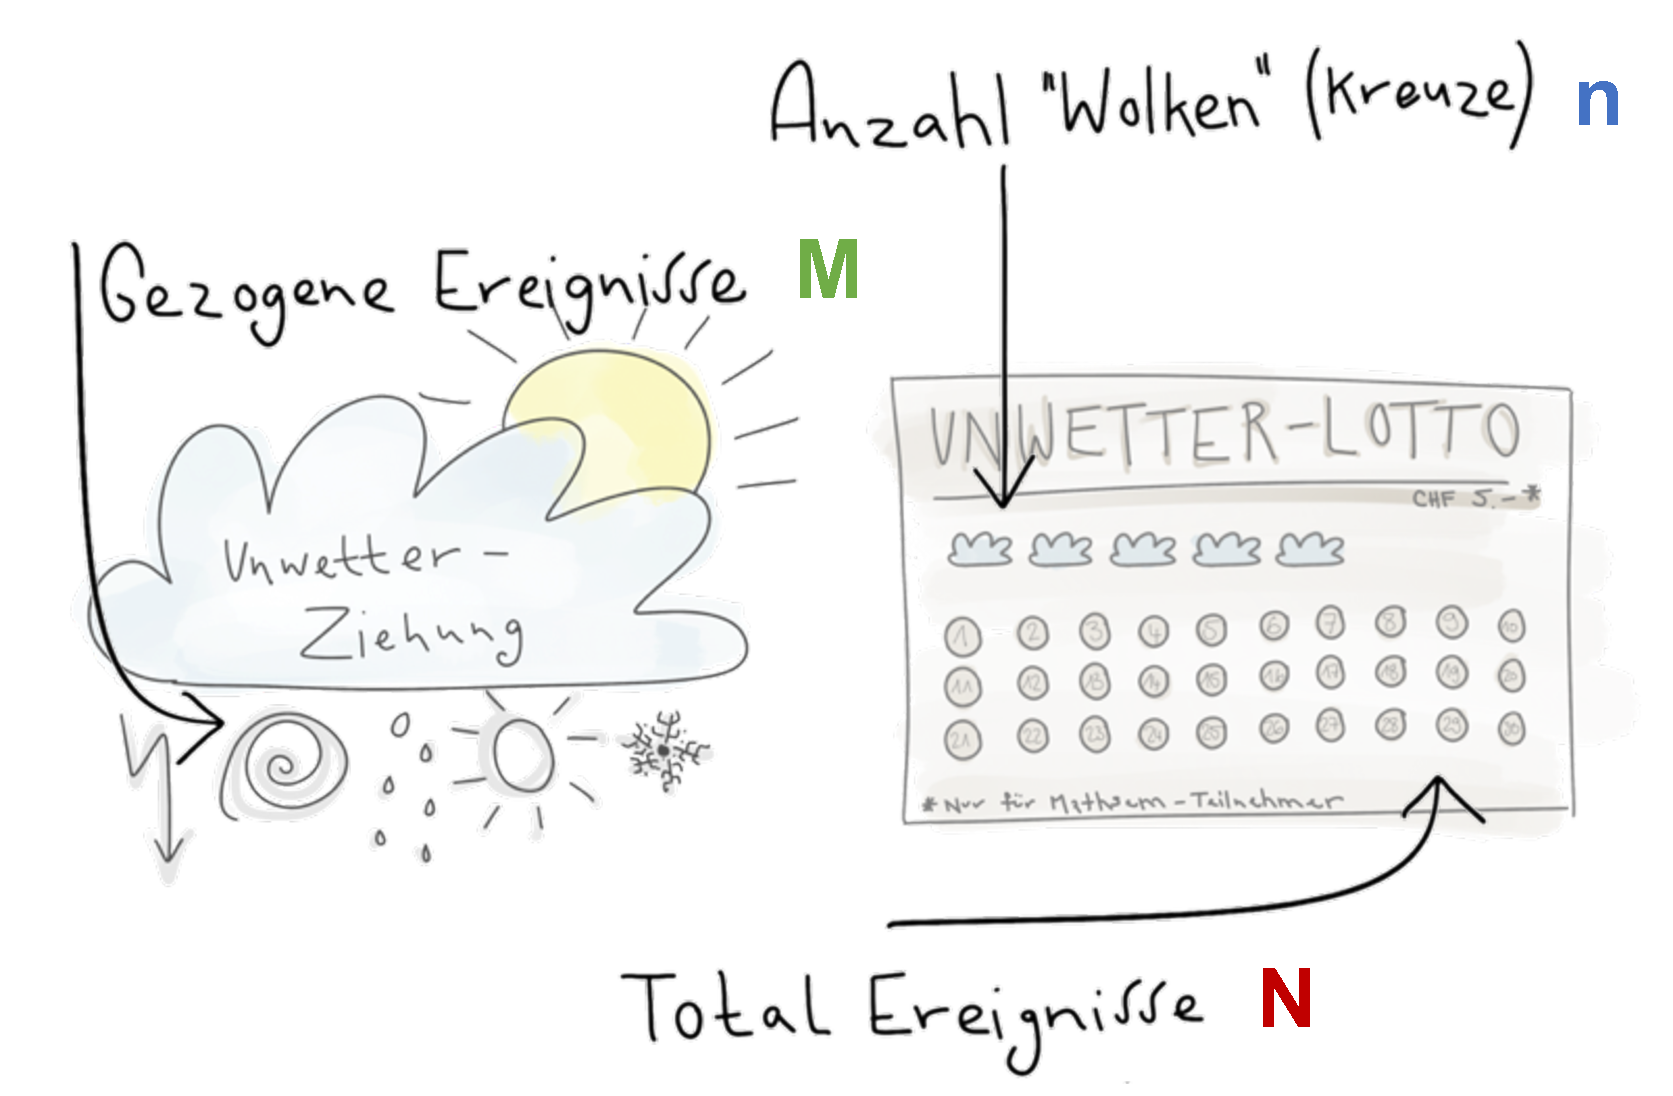
\includegraphics[width=0.6\textwidth]{extrem/Lottoscheinausgefuellt.pdf}
\caption{Unwetterlottoschein mit den Variabeln und der Unwetterziehung.}
\label{Lottoscheinausgefuellt}
\end{figure}

\begin{figure}
\centering
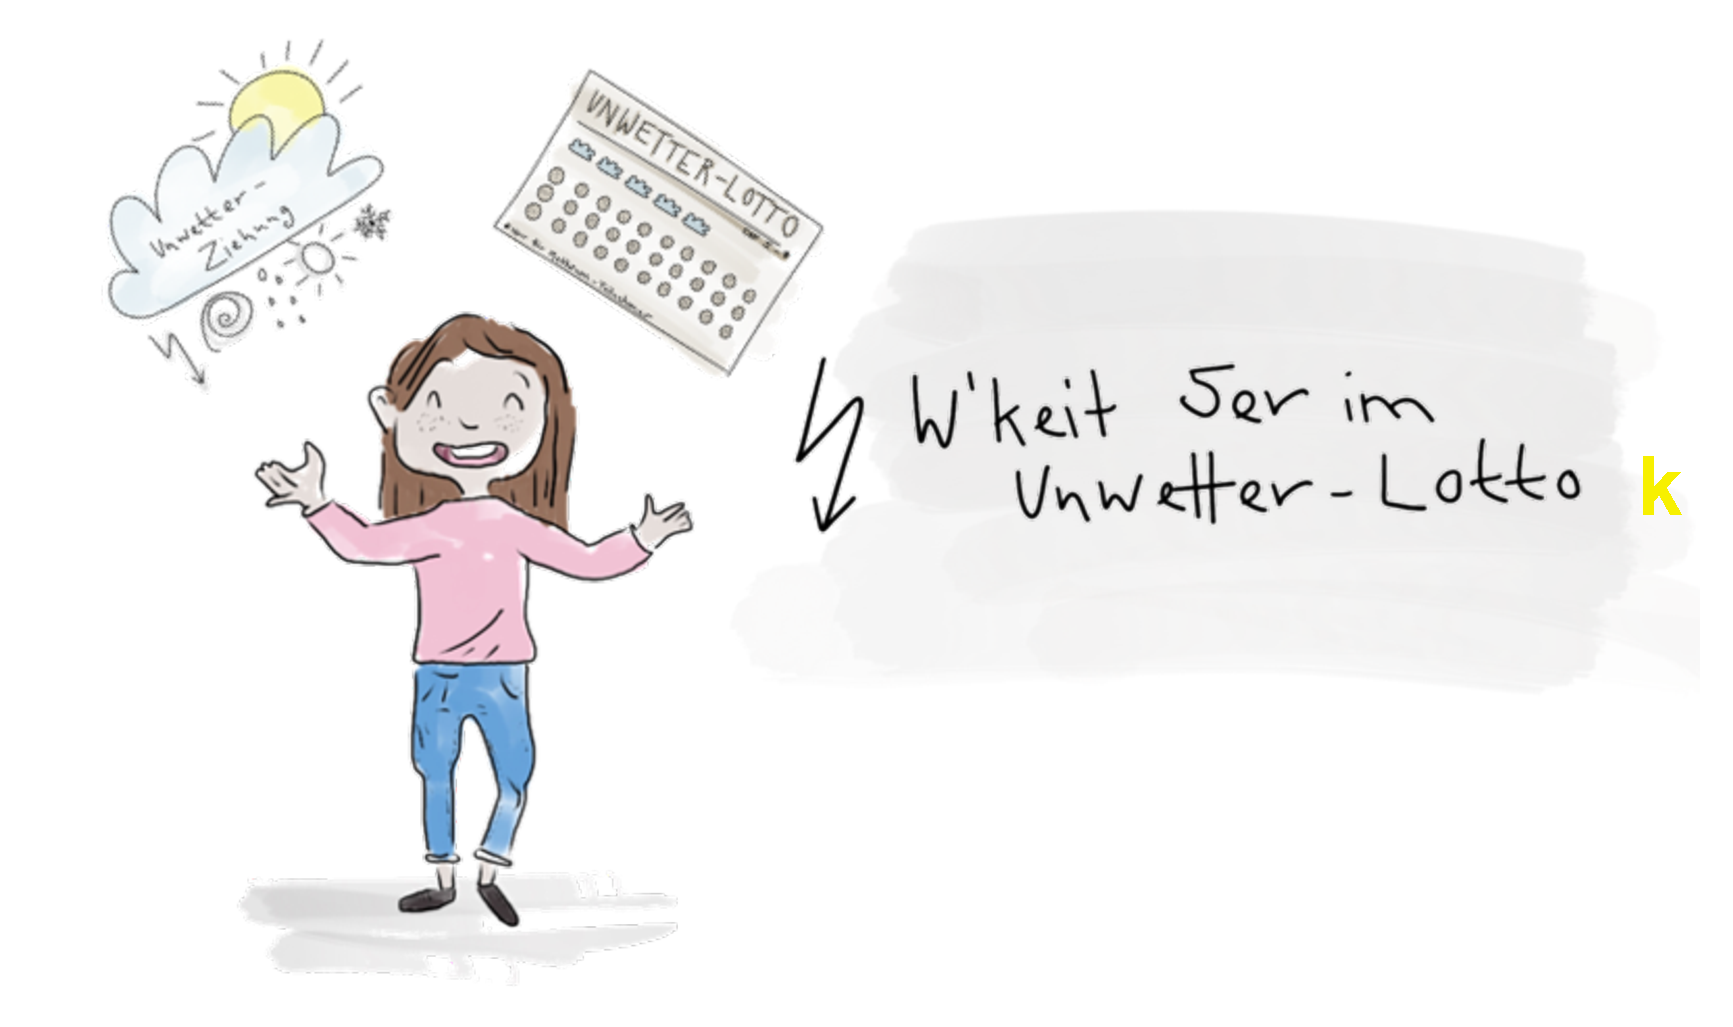
\includegraphics[width=0.6\textwidth]{extrem/wkeitlotto.pdf}
\caption{Wahrscheinlichkeit, einen 5er im Unwetterlotto zu erhalten.}
\label{WahrscheinlichkeitUnwetterlotto}
\end{figure}

\subsection{Lottoproblem} \label{Lottoproblem}
Mit dem Unwetterlotto wurde das bekannte Lottoproblem beschrieben - ein Experiment ohne zurücklegen. Mit jeder Ziehung ändert sich im Laufe des Experiments die Grundgesamtheit und somit auch die Wahrscheinlichkeit ein bestimmtes Ereignis zu ziehen. Der Ziehmodus ist vorgegeben und somit ist auch der Gewinn bekannt.
Das oben beschriebene Lottoproblem liefert uns folgende Fragestellung:


Wie wahrscheinlich ist es...

\begin{itemize}
\item \dots auf einem Lottozettel mit \textcolor{red}{\textbf{N}} Feldern \dots
\item \dots auf welchem man \textcolor{blue}{\textbf{n}} Unwetter ankreuzen kann \dots
\item \dots und bei der Ziehung \textcolor{green}{\textbf{M}} Unwetter gezogen werden \dots
\item \dots genau \textcolor{yellow}{\textbf{k}} Richtige zu haben?
\end{itemize}


\section{Die Unwetter-Verteilung}
Um die Frage zu beantworten, ob sich das Klima verändert und ob immer häufiger extreme Ereignisse auftreten, bedienen wir uns aus dem Werkzeugkasten der Statistik. Mit dem genannten ~\ref{Lottoproblem} \nameref{Lottoproblem}, lässt sich die Unwetter-Verteilung aufstellen.

Dabei beziehen sich die \textcolor{red}{\textbf{N}} Felder auf dem Lottozettel auf die Anzahl Jahre mit zugehörigen Messwerten. Die Anzahl Unwetter \textcolor{blue}{\textbf{n}} welche man ankreuzen kann, sind die extremen Ereignisse, also Unwetter oder Messungen welche besonders extrem ausgefallen sind. Die Ziehung der \textcolor{green}{\textbf{M}} Unwetter ist unser Beobachtungszeitraum. Im nachfolgenden Abschnitt ~\ref{Beispiel} \nameref{Beispiel} wird ein Beobachtungszeitraum von 10 Jahren angenommen.


Die Frage welche nun beantwortet werden muss lautet:
Wie wahrscheinlich (\textcolor{yellow}{\textbf{k}}) ist es, dass \textcolor{blue}{\textbf{n}} extreme Ereignisse aus einer Messreihe von \textcolor{red}{\textbf{N}} Jahren, in den letzten 10 Jahren (\textcolor{green}{\textbf{M}}) vorkommen?


%\begin{figure}
%\centering
%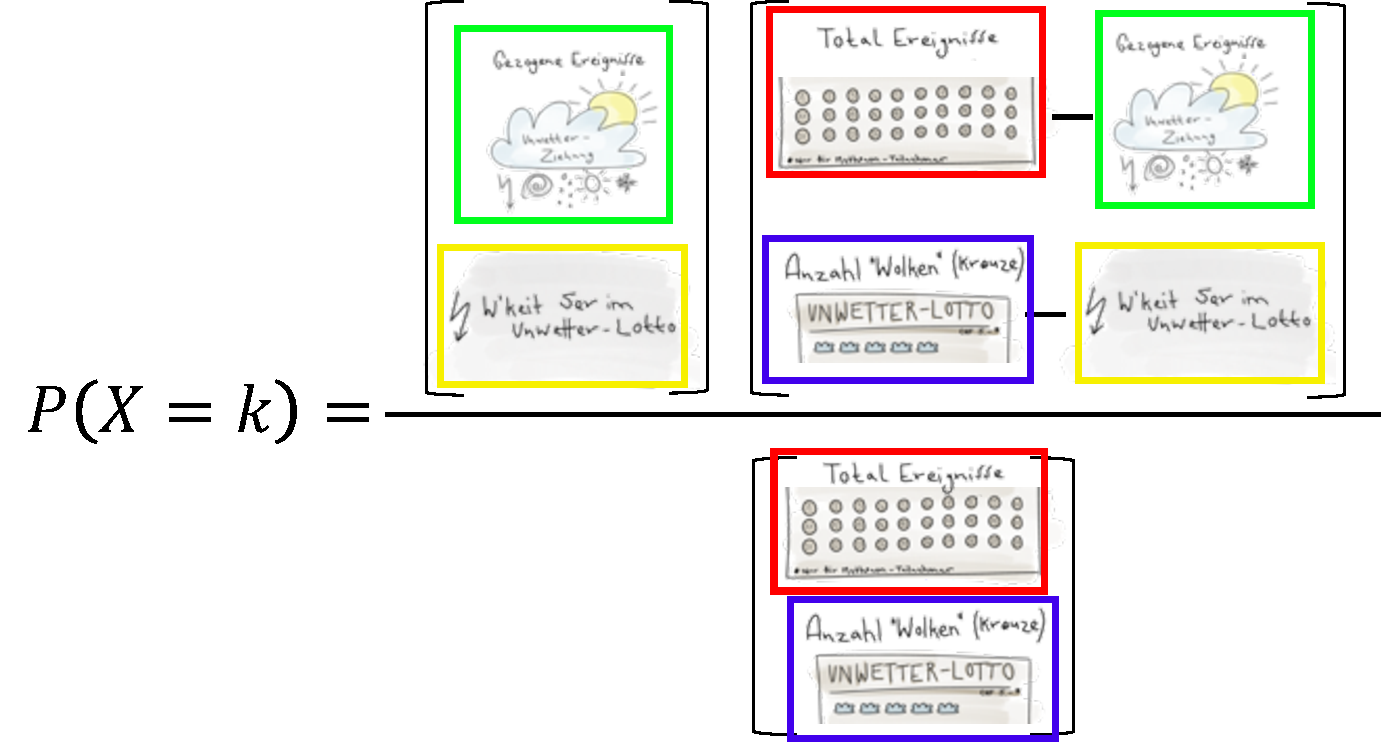
\includegraphics[width=0.8\textwidth]{extrem/Unwettervert.pdf}
%\caption{Unwetterverteilung mit den Ereignissen ergeben die Wahrscheinlichkeit %für die Anzahl treffer.}
%\label{UnwetterVerteilung}
%\end{figure}


Die Unwetter-Verteilung ist somit nichts anderes als die hypergeometrische Verteilung. Die hypergeometrische Verteilung

\begin{align*}
P(X = k) = 
\frac{\displaystyle \binom{M}{k} \binom{N-M}{n-k}}{\displaystyle \binom{N}{n} }
\end{align*}

beschreibt die Wahrscheinlichkeit aus $N$ gegebenen Elementen, mit $n$ Elementen einer speziellen Eigenschaft, und einer Stichprobe aus $M$ Elementen genau $k$ Treffer zu erzielen. 
Anders als die Binomialverteilung ist die hypergeometrische Verteilung ein Experiment ohne zurücklegen. Die Wahrscheinlichkeit ändert sich mit jeder Ziehung. Die Frage wie wahrscheinlich (k) es ist, dass n extreme Ereignisse aus einer Messreihe von N Jahren in den letzten 10 Jahren (M) vorkommt, kann nun beantwortet werden.


\subsection{Beispiel} \label{Beispiel}
Die hypergeometrische Verteilung setzt sich aus verschiedenen Binomialkoeffizienten

\begin{align*}
\binom{n}{k} = \frac {n!}{k! \cdot (n-k)!} 
\end{align*}
zusammen.

Um in ~\ref{MesspunkteSchweiz} \nameref{MesspunkteSchweiz} die Klimadaten auszuwerten, werden im nachfolgenden Beispiel der hypergeometrischen Verteilung die folgenden Werte für die entsprechenden Variabeln verwendet:
\begin{align*}
N = 75 \quad \quad \quad \quad \quad \quad 
n = 7 \\
M = 10 \quad \quad \quad \quad \quad \quad 
k = 3
\end{align*}

Die Wahrscheinlichkeit P (X = 3) ergibt sich aus:
Anzahl der Möglichkeiten, genau 3 extreme Ereignisse (und damit genau 4 normale) Ereignisse auszuwählen, dividiert durch die Anzahl Möglichkeiten 7 Ereignisse aus allen Ereignissen auszuwählen.
 
Dabei gibt es
\begin{align*}
\binom{M}{k} = \binom{10}{3} = 120
\end{align*}

Möglichkeiten, genau 3 extreme Ereignisse auszuwählen.
Zudem gibt es 
\begin{align*}
\binom{N-M}{n-k} = \binom{75-10}{7-3} = \binom{65}{4} = 677040
\end{align*}

Möglichkeiten, genau 4 normale Ereignisse auszuwählen.
Da jede Möglichkeit 3 extreme Ereignisse mit jeder Möglichkeit 4 normale Ereignisse auszuwählen kombiniert werden kann, ergibt sich
\begin{align*}
\binom{M}{k} \cdot \binom{N-M}{n-k} = \binom{10}{3} \cdot \binom{75-10}{7-3} = 120 
\cdot 677040 = 81244800
\end{align*}

Möglichkeiten für genau 3 extreme und 4 normale Ereignisse auszuwählen.
Zusätzlich gibt es insgesamt
\begin{align*}
\binom{N}{n} = \binom{75}{7} = 1984829850
\end{align*}

Möglichkeiten, 7 Ereignisse aus allen Ereignissen zu ziehen.
Für k = 3 erhalten wir somit die Wahrscheinlichkeit
\begin{align*}
P(X = 3) &= \frac{\displaystyle \binom{M}{k} \binom{N-M}{n-k}}{\displaystyle \binom{N}{n} }  \\
&= \frac{\displaystyle \binom{10}{3} \binom{75-10}{7-3}}{\displaystyle \binom{75}{7} } \\
&= \frac{ 120 \cdot 677040}{ 1984829850 } = 0.0409329
\end{align*}

In rund 4.09 \% aller Fälle werden genau 3 extreme und 4 normale Ereignisse vorkommen. Diese Berechnung lässt sich mit allen $X=k$ durchführen, dies wird im Kapitel ~\ref{Dichtehyper} \nameref{Dichtehyper} gemacht.


\subsection{Die hypergeometrischen Verteilung} \label{Dichtehyper}
Im vorangehenden Beispiel wurde die Wahrscheinlichkeit der hypergeometrischen Verteilung berechnet für $f(k = 3)$. 

\begin{definition}
Die hypergeometrischen Verteilung, sind die Wahrscheinlichkeitswerte für alle P(X = k).
\end{definition}

Für alle $P (X=k)$ ergeben sich folgende Wahrscheinlichkeiten (Abbildung \ref{TabHyper}).

%\begin{figure}
%\centering
%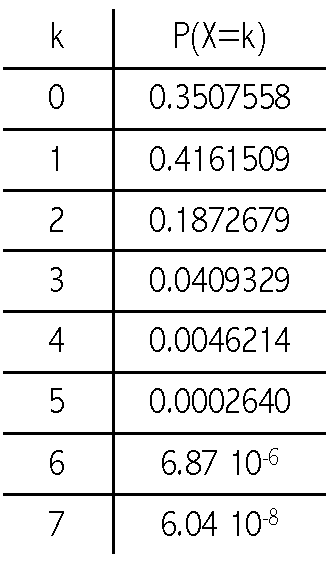
\includegraphics[width=0.2\textwidth]{extrem/TabHyper.pdf}
%\caption{Wahrscheinlichkeiten P (X=k) der verschiedenen Ereignisse.}
%\label{TabHyper}
%\end{figure}

Die Wahrscheinlichkeit beschreibt dabei, wie wahrscheinlich es ist, genau k extreme Ereignisse in den letzten 10 Jahren vor zufinden.
Beachte, dass die Werte N, M und n das Experiment beschreiben und nicht mehr verändert werden. Die Variable k hingegen kann alle möglichen Ausgänge des Experiments annehmen, in unserem Beispiel also von 0 bis 7.

%\begin{figure}
%\centering
%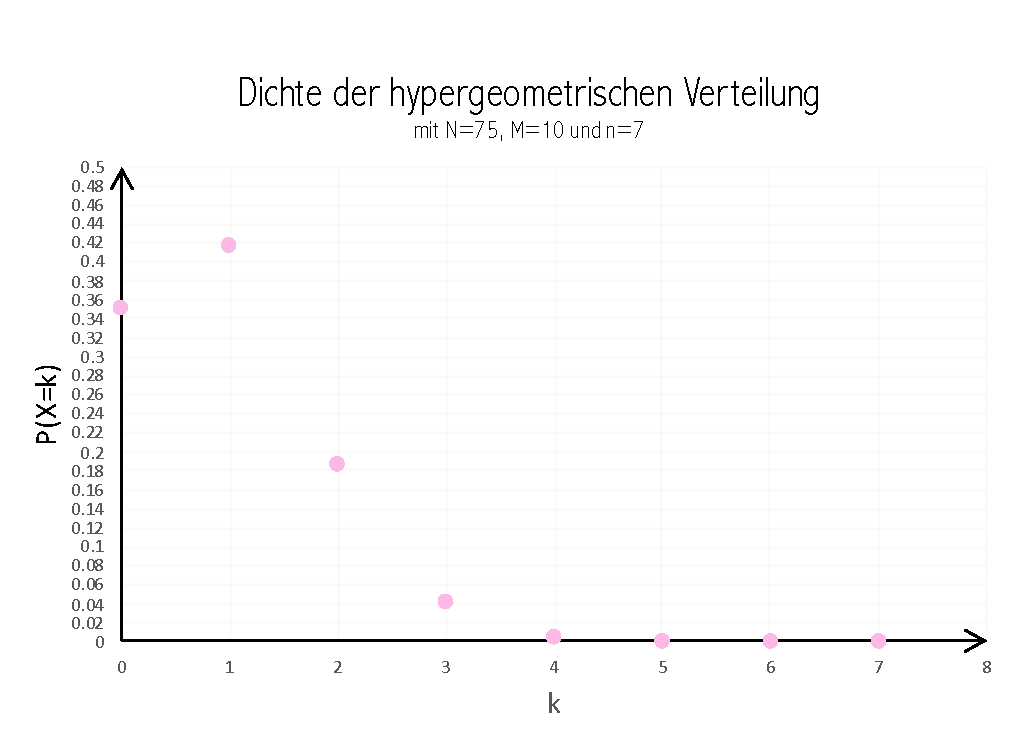
\includegraphics[width=0.8\textwidth]{extrem/Hyper.pdf}
%\caption{Die hypergeometrische Verteilung unseres Beispiels. Sie zeigt auf, wie %wahrscheinlich es ist, genau k extreme Ereignisse in den letzten 10 Jahren %vorzufinden.}
%\label{Hyper}
%\end{figure}

In Abbildung \ref{Hyper} ist sehr gut ersichtlich, dass die Wahrscheinlichkeit bei genau einem extremen Ereignis in den letzten 10 Jahren am höchsten ist. Wohingegen genau 3 Ereignisse nur noch eine Wahrscheinlichkeit von 4.09\% aufweisen, was bereits sehr unwahrscheinlich ist. Häufungen von Ereignissen, welche die Anzahl 3 überschreiten, sind so unwahrscheinlich, das sie kaum natürlichen Ursprungs sein können.

\subsection{Sind viele extreme Ereignisse wahrscheinlich?}
Stellt man sich nun die Frage ob viele extreme Ereignisse wahrscheinlich sind, muss berechnet werden wie wahrscheinlich es ist k oder mehr Ereignisse in den letzten 10 Jahren (M) zu erhalten. 
Die Verteilungsfunktion der hypergeometrischen Verteilung ist nichts anderes, als die Aufsummierte Wahrscheinlichkeit aller möglichen Ausgänge. Weil für unser Beispiel aber wichtig ist wie wahrscheinlich es ist, drei oder mehr extreme Ereignisse in den letzten 10 Jahren vorzufinden, muss die Komplementäre Verteilungsfunktion 

\begin{align*}
F(x) = P(X \ge I ) = \(\sum \limits_{k=I}^n P(X = k)) 
\end{align*}

angeschaut werden.


Möchten wir also die Wahrscheinlichkeit wissen, drei oder mehr extreme Ereignisse in den letzten 10 Jahren vorzufinden, müssen die einzelnen Wahrscheinlichkeiten aufsummiert werden:

\begin{align*}
\bar{F}(3) &=  P(X {\ge} 3) \\
&= P(X = 3) + P(X = 4) + P(X = 5) + P(X = 6) + P(X = 7) \\
&= 0.0409329 + 0.0046214 + 0.00026340 + 6.87 10^{ -6 } + 6.04 10^{ -8 } \\
&= 0.045833 \quad  4.58\%
\end{align*}

Drei oder mehr extreme Ereignisse in den letzten 10 Jahren sind mit einer Wahrscheinlichkeit von 4.58\% möglich. 
Die Wahrscheinlichkeit ein oder zwei extreme Ereignisse in den letzten 10 Jahren zu haben ist mit 64.49\% und 23.30\% relativ hoch. Ab drei oder mehr Ereignissen nimmt die Wahrscheinlichkeit rasant ab. Ohne Äussere Einwirkungen sind drei oder mehr Ereignisse sehr unwahrscheinlich und ab 5 nahezu unmöglich.

%\begin{figure}
%\centering
%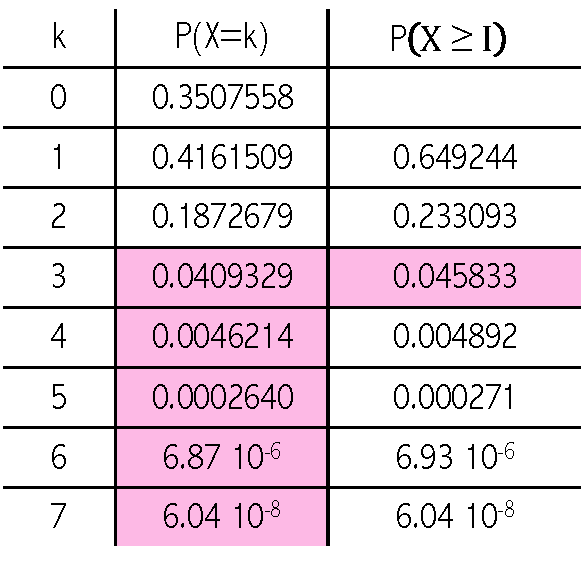
\includegraphics[width=0.3\textwidth]{extrem/TabExt.pdf}
%\caption{Wahrscheinlichkeit $P(X \ge I)$ aller Ereignisse unseres Beispiels. %Rosa markiert ist das oben berechnete Beispiel mit drei oder mehr extremen %Ereignissen in den letzten 10 Jahren. }
%\label{TabExt}
%\end{figure}

\begin{figure}
\centering
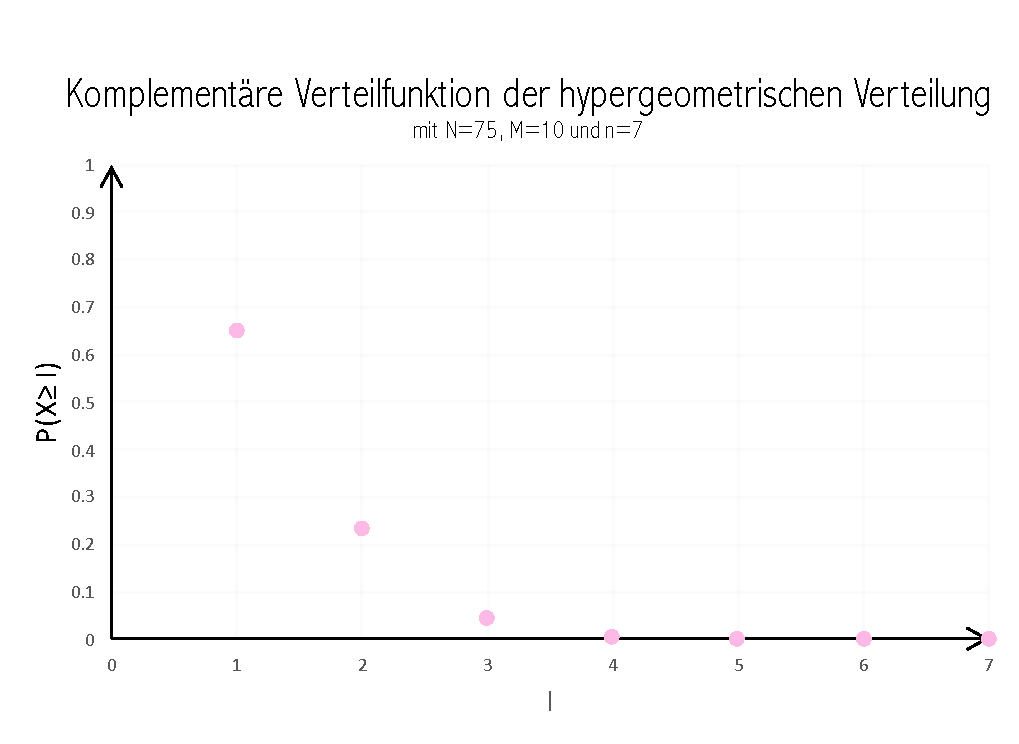
\includegraphics[width=0.8\textwidth]{extrem/HyperExt.pdf}
\caption{Die komplementäre Verteilfunktion $F(x)$ der hypergeometrischen Verteilung zeigt auf, wie wahrscheinlich es ist mehr als k Ereignisse in den letzten 10 Jahren vorzufinden.}
\label{HyperExt}
\end{figure}




\section{Hypothesentest}
Hypothesentests werden immer dann durchgeführt, wenn man aus erhobenen Daten etwas nachweisen möchte, zum Beispiel das sich extreme Ereignisse in den letzten Jahren häufen. Der Grundsatz bei allen statistischen Tests ist, das wir das Gegenteil widerlegen müssen - wir müssen also widerlegen, dass extreme Ereignisse in den letzten Jahren zufällig verteilt sind. Das heisst die Häufung von extremen Ereignissen entscheidet der Zufall und kann nicht beeinflusst werden.

Zu vergleichen ist ein Hypothesentest mit einer Gerichtsverhandlung. Im Zweifel ist das Gericht für den Angeklagten. Es muss davon ausgegangen werden, dass die Hypothese stimmt, auch wenn man es nicht weiss bis das Gegenteil bewiesen werden kann. Hierfür benötigt es genügend Beweise, welche die Schuld oder hier die Hypothese widerlegen, ohne das Zweifel aufkommen können. Falls ungenügend viele Beweise vorliegen, muss davon ausgegangen werden, dass die Hypothese stimmt oder eben der Angeklagte unschuldig ist.
Zuerst wird die Nullhypothese aufgestellt, welche das Gegenteil besagt von dem zu beweisenden Ziel.

\subsection{Nullhypothese}
Unsere Nullhypothese welche geprüft werden soll:

In den letzten Jahren gab es keinen Wandel oder eine Häufigkeit von extremen Ereignissen. 

Zusammengefasst:
\begin{itemize}
\item Das Klima verändert sich nicht
\item Alles bleibt beim alten
\item Der Zufall bestimmt die Anordnung der (extremen) Ereignisse
\end{itemize}

Diese Nullhypothese muss nun widerlegt werden, um den Klimawandel zu beweisen.

\subsection{Signifikanzniveau}
Die Grenze für die Widerlegung der Nullhypothese beschreibt die statistische Signifikanz $\alpha$. Über diesen Wert wird eine bestimmte Irrtumswahrscheinlichkeit festgelegt.
Bei der Festlegung dieser Schwelle wird bedacht, was für Konsequenzen es hätte, das ein beobachteter Unterschied nur zufällig erfolgt. Sind die Folgen gravierend, wählt man eher ein tiefes Niveau (1 \% statt 5\%).

Bei einem Medikament wird daher eher ein tiefes Signifikanzniveau gewählt. Als Vergleich, beim Nachweis der Existenz des Higgs-Bosons\footnote{%
Das Higgs-Boson ist Elementarteilchen (Benannt nach dem britischen Physiker Peter Higgs), deren Existenz wurde im Juli 2012 durch das CERN (mit dem Larce Hadron Collider LHC) bestätigt.} wurde ein noch viel strengeres Kriterium gewählt, es entspricht einem Wert von 1 in 3.5 Millionen. Da extreme Ereignisse nicht direkt Lebensbedrohlich sind, wird im Folgenden $\alpha$ = 5\% gewählt.
Falls die Nullhypothese richtig ist, darf die Wahrscheinlichkeit dafür, dass sie fälschlicherweise abgelehnt wird, nicht unter 5\% fallen.
In unserem Beispiel bedeutet das:

%\begin{figure}
%\centering
%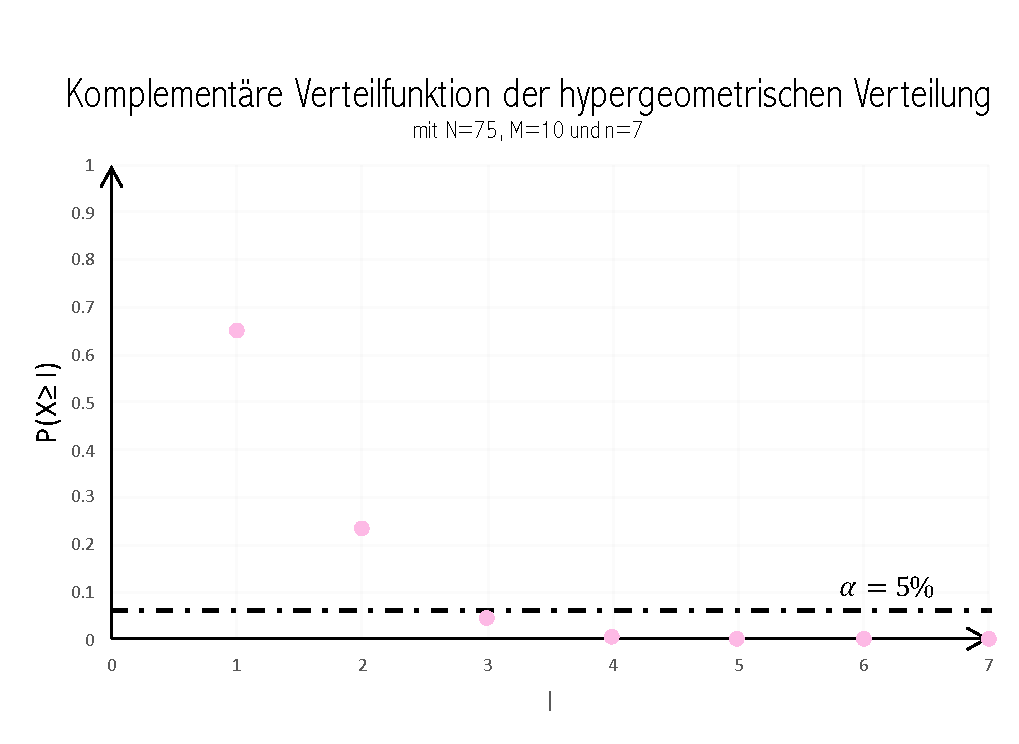
\includegraphics[width=0.8\textwidth]{extrem/Signi.pdf}
%\caption{Die komplementäre Verteilfunktion der hypergeometrischen Verteilung %mit dem Signifikanzniveau $\alpha = 5%$.}
%\label{Signifikanzniveau}
%\end{figure}

Eine Häufung von 3 oder mehr extremen Ereignissen wären nicht mehr durch den Zufall bestimmt. 

Konkret: Wenn von den 7 extremsten Ereignissen der letzten 75 Jahre 3 oder mehr in den letzten 10 Jahren waren, müssen wir auf den Klimawandel schliessen.


\section{Messpunkte Schweiz} \label{MesspunkteSchweiz}
Um eine möglichst grosse Vielfalt von Messreihen zu bekommen, werden verschiedene Messpunkte in der Schweiz angeschaut. 

\begin{figure}
\centering
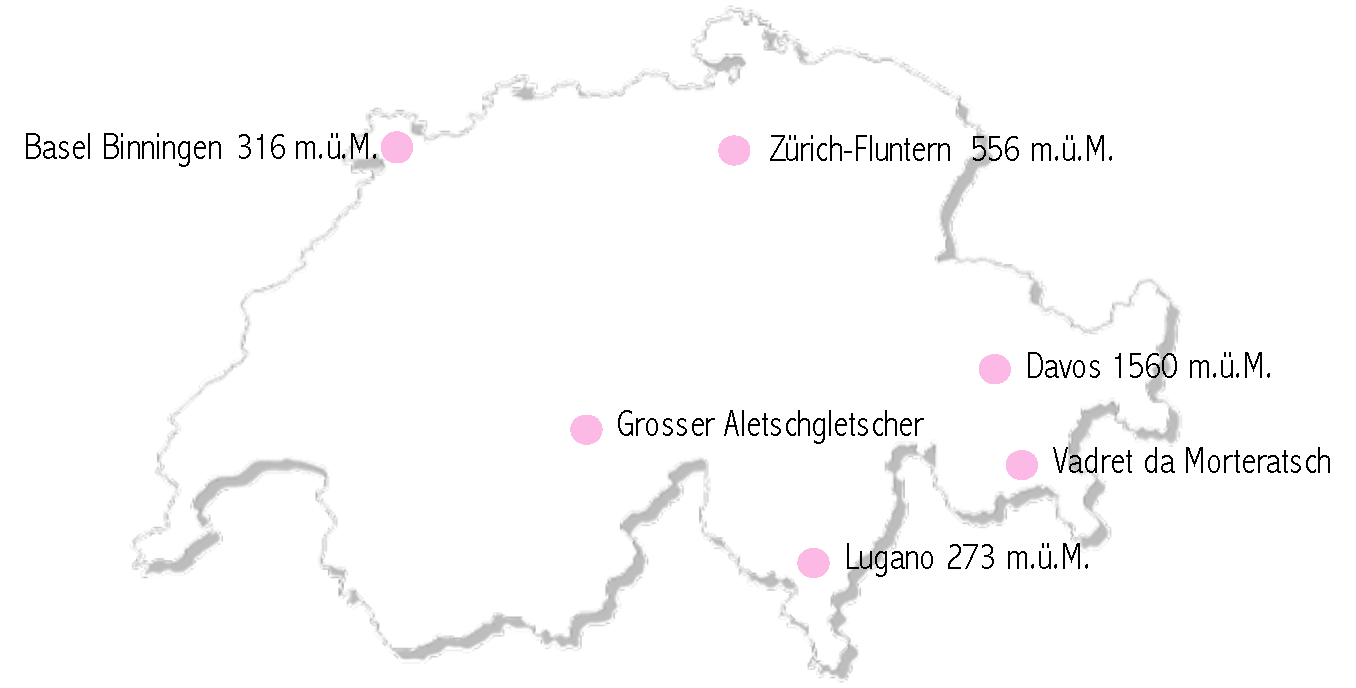
\includegraphics[width=0.8\textwidth]{extrem/Schweiz.pdf}
\caption{Gewählte Messpunkte in der Schweiz.}
\label{MesspunkteSchweiz}
\end{figure}

Die Messreihen der Standorte Basel Binningen, Zürich-Fluntern, Lugano und Davos sind von MeteoSchweiz und sind öffentlich zugänglich. Die Daten sind bereits homogenisiert.
Die Messdaten der Gletscher werden vom Schweizerischen Gletschermessnetz GLAMOS \footnote{%
Die Veränderungen der Schweizer Gletscher werden jährlich gemessen. Das Messnetz GLAMOS wird getragen durch die ETH Zürich und die Universitäten Fribourg und Zürich mit finanzieller Unterstützung durch das Bundesamt für Umwelt BAFU, MeteoSchweiz und SCNAT.} ebenfalls öffentlich zugänglich zur Verfügung gestellt.


\subsection{Prüfung Messreihe}
Die Messreihen geben einen Einblick über die letzten 74 Jahre, nämlich von 1943 -- 2017. Damit die Hypothese widerlegt wird und somit der Klimawandel nachgewiesen werden kann, müssen drei oder mehr extreme Ereignisse in den letzten 10 Jahren vorkommen (Abbildung \ref{TabExt}). Dann wäre das Signifikanzniveau $\alpha$ von 0.05 unterschritten und die Hypothese ohne jegliche Zweifel widerlegt.


\section{Temperatur}
Die Jahresmitteltemperatur in der Schweiz ist seit 1864 rund $2^{\circ}$ gestiegen (Stand 2018, MeteoSchweiz). Der grösste Anstieg passierte in den letzten Jahrzehnnten. Dennoch ist für die breite Bevölkerung ein Anstieg von $2^{\circ}$ schwierig nachzuvollziehen.
In den nachfolgenden Beispielen, wurden Klimaindikatoren gewählt, welche jeder kennt und beobachtet werden können.

\subsection{Jahres Mitteltemperatur}
Die Jahres Mitteltemperatur ist wie folgt definiert

\begin{definition}
Mittlere Jahrestemperatur in $^{\circ}$C.
\end{definition}

Bei der Jahresmitteltemperatur ist das Ergebnis eindeutig (Abbildung \ref{JMittel}). Bei beiden Messpunkten, sowohl Lugano als auch Basel Binningen, wird der Hypothesentest widerlegt da die Alphagrenze unterschritten wird. Bei Basel Binningen kommen vier der extremsten Ereignisse in den letzten 10 Jahren vor. In Lugano sind es sogar deren fünf! 


\subsection{Sommertage}
Ein Sommertag ist wie folgt definiert

\begin{definition}
Maximale Temperatur $\ge 25^{\circ}$C und langjähriger Mittelwert (1961 - 1990).
\end{definition}

Die Sommertage in Lugano waren in den letzten 10 Jahren nie extrem. Zu Beginn der Messungen um die Jahre 1943-1959 zeigen sich Extremwerte. Wohingegen Davos eine Häufung der Anzahl von Sommertagen in den letzten 10 Jahren zeigt. In den früheren Messjahren waren keine oder nur sehr wenige Sommertage vorhanden. In en letzten 10 Jahren ist die Anzahl aber immer weiter gestiegen und ist mit 5 Ereignissen nahezu unmöglich. In Davos wird die Hypothese widerlegt und somit ein Wandel im Klima nachgewiesen.


\subsection{Tropennächte}
Eine Tropennacht ist wie folgt definiert

\begin{definition}
Minimale Temperatur $\ge 20^{\circ}$C und langjähriger Mittelwert (1961 -- 1990).
\end{definition}

Sowohl in Lugano wie auch Basel Binningen sind in den letzten 10 Jahren eine extreme Anzahl von Tropennächten gemessen worden. Mit vier Ereignissen pro Standort wird das Signifikanzniveau deutlich unterschritten.


\subsection{Hitzetage} \label{Hitzetage}

Ein Hitzetag ist wie folgt definiert

\begin{definition}
Maximale Temperatur $\ge 30^{\circ}$C und langjähriger Mittelwert (1961 -- 1990).
\end{definition}

Bei den Hitzetagen ist im Klima kein Wandel zu erkennen. Weder in Zürich-Fluntern noch in Lugano wurden in den letzten Jahren extrem viele Hitzetage gemessen. Bei beiden Orten, waren die Hitzetage zu Beginn der Messreihe (um 1943) vermehrt vorgekommen.


\subsection{Frosttage}
Ein Frosttag ist wie folgt definiert

\begin{definition}
Minimale Temperatur $< 0^{\circ}$C und langjähriger Mittelwert (1961 -- 1990).
\end{definition}

Wie bereits bei den Hitzetagen ~\ref{Hitzetage} \nameref{Hitzetage} ist auch bei den Frosttagen weder in Basel Binningen noch in Lugano kein Wandel im Klima zu erkennen. Ebenso wurden die Extreme vermehrt zu Beginn der Messreihe gemessen.


\subsection{Eistage}
Ein Eistag ist wie folgt definiert

\begin{definition}
Maximale Temperatur $< 0^{\circ}$C und langjähriger Mittelwert (1961 -- 1990).
\end{definition}

Anhang der Anzahl Eistage in Zürich-Fluntern und Davos, kann kein Klimawandel festgestellt werden. Weder in den oberen noch in den unteren Extremen Ereignissen.


\section{Niederschlag}
In den letzen Jahren nahmen die Niederschläge zu. Vor allem in den Jahren XY kam es zu Hochwasserereignissen in der ganzen Schweiz. Ausuferungen, Überschwemmungen und Schlammlawinen waren folgen von diesen heftigen Unwettern. Die Schadensumme belief sich im Jahr XY auf CHF .... Millionen Schweizer Franken. 

\subsection{Jahresniederschlag}
Der Jahresniederschlag ist wie folgt definiert

\begin{definition}
Jahresniederschlag in mm.
\end{definition}

Der Jahresniederschlag hat in den letzten Jahren zwar zugenommen, zeigt aber keine Häufung von extremen Ereignissen in den letzten 10 Jahren. Anhand des Jahresniederschlag kann man nicht auf den Klimawandel schliessen.


\subsection{Neuschnee}
Die Neuschneemenge ist wie folgt definiert

\begin{definition}
Neuschneemenge, Jahressumme der täglichen Aufzeichnung in cm.
\end{definition}

Ähnlich sieht es bei den Neuschneemengen aus. Weder bei extrem viel gefallenen Neuschnee, noch bei extrem wenig gefallenem Neuschnee ist ein Klimawandel zu erkenne. Hier wäre ebenfalls die Fragestellung anzupassen und zu analysieren wie lange der Schnee liegen bleibt.


\section{Gletscher}
Bei den Gletscherdaten wurde ein Zeitraum von 1881 - 2017 gewählt. Durch die Anzahl der Messjahre verschieben sich die Wahrscheinlichkeiten der Ereignisse. In den Beispielen der Gletscher müssen aber ebenso 3 oder mehr extreme Ereignisse in den letzten 10 Jahren vorkommen um diese dem Klimawandel zuschreiben zu können.

\subsection{Grosser Aletschgletscher}
Der grosse Aletschgletscher schmilzt, wie man gut auf der (Abbildung \ref{Aletsch}) sehen kann. Jedoch zeigen die Messwerte der letzen 136 Jahren keinen extremen Schwund der Eismassen auf.

\begin{figure}
\centering
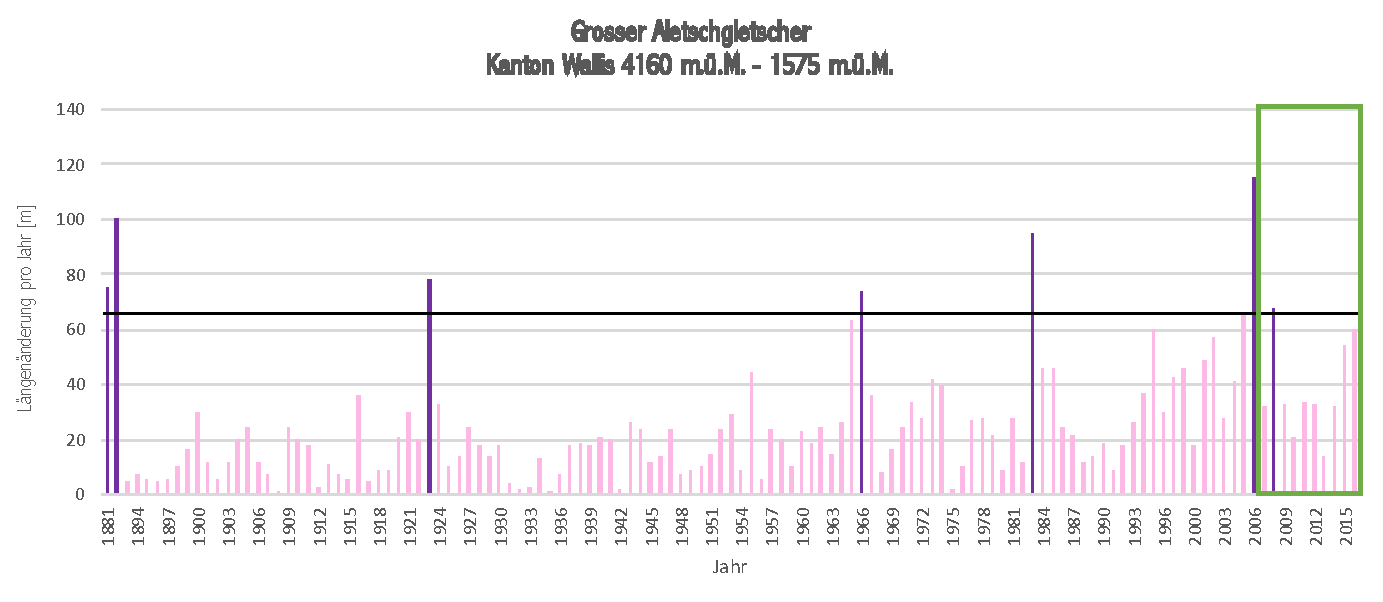
\includegraphics[width=1.0\textwidth]{extrem/Aletsch.pdf}
\caption{DBLaBLa}
\label{AletschTab}
\end{figure}

Hier müsste die Messreihe hinterfragt werden. Die Messreihe zeigt nur die Längenänderung pro Jahr auf, wieviel die Gletscherzunge schwindet und nicht die Volumenänderung der Eismasse. Der Gletscher könnte in der Länge nur wenig schwinden würde aber im selben Jahr sehr viel an Volumen verlieren, wäre dies dennoch nicht in der Messreihe ersichtlich.

\begin{figure}
\centering
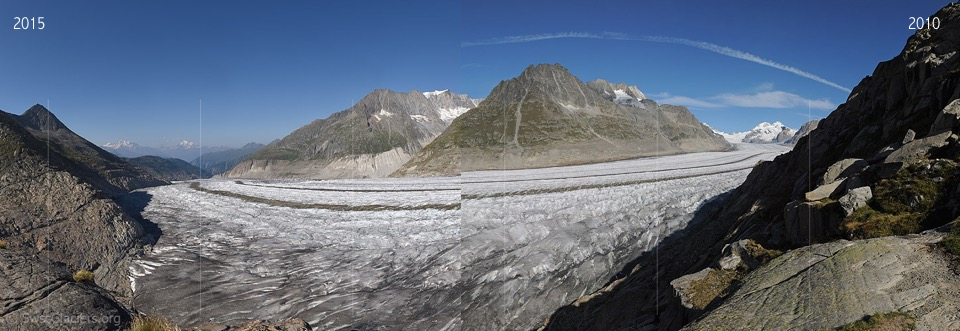
\includegraphics[width=1.0\textwidth]{extrem/Aletsch.jpg}
\caption{Der grosse Aletschgletscher im Wandel der Zeit. Links im Jahr 2015 und rechts im Jahr 2010.}
\label{Aletsch}
\end{figure}


\subsection{Vadret da Morteratsch}
Beim Morteratschgletscher sieht es anders aus. Die Längenänderung in den letzten 10 Jahren ist massiv. Hier kann aufgrund der extremen Längenänderung auf den Klimawandel geschlossen werden. Dies ist auch deutlich in der (Abbildung \ref{Morteratsch}) ersichtlich.


\begin{figure}
\centering
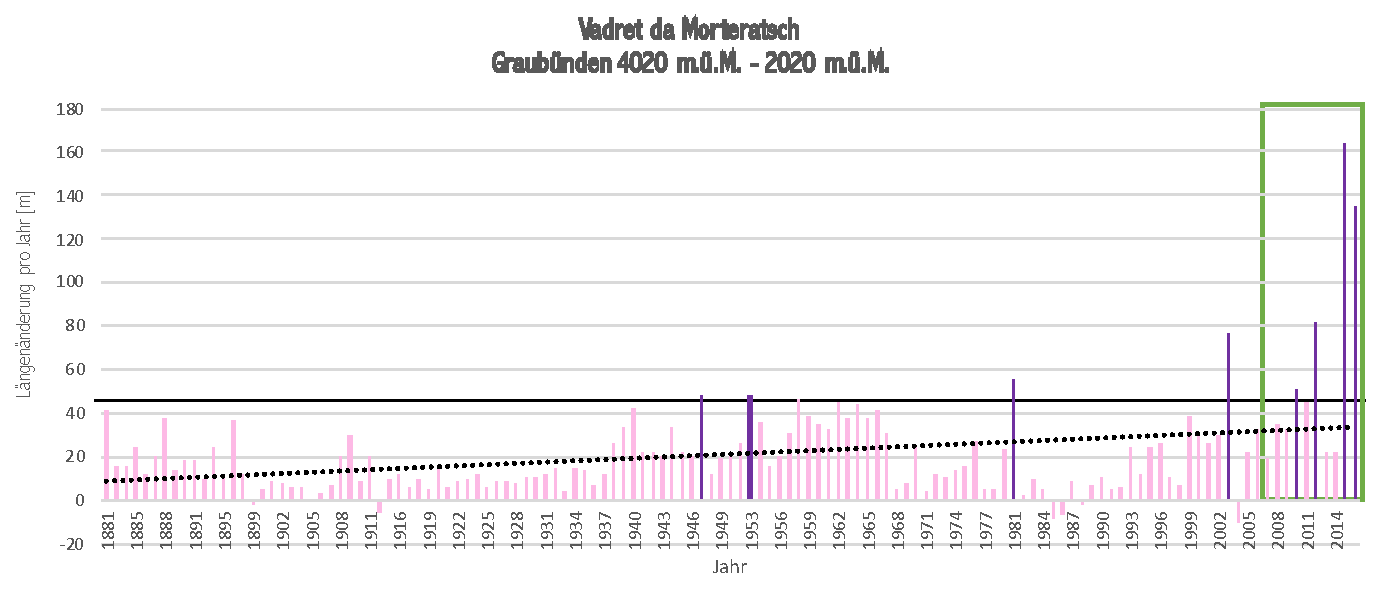
\includegraphics[width=1.0\textwidth]{extrem/Morteratsch.pdf}
\caption{BlaBla}
\label{Morteratschtab}
\end{figure}


\begin{figure}
\centering
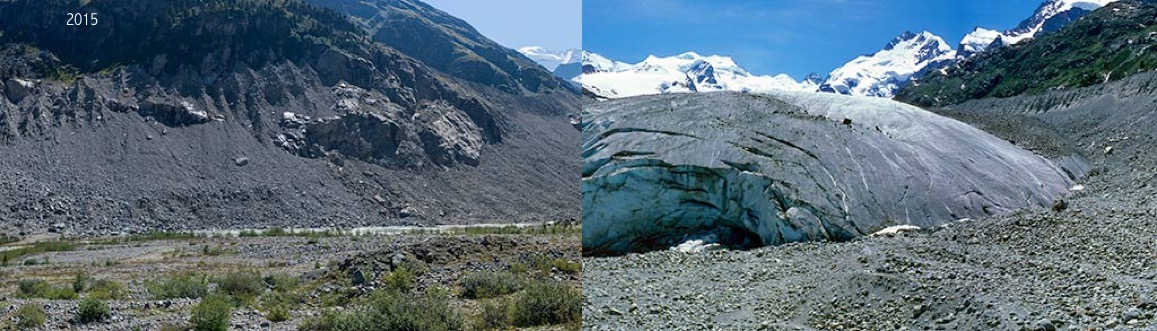
\includegraphics[width=1.0\textwidth]{extrem/Morteratsch.jpg}
\caption{Der Morteratschgletscher im Wandel der Zeit. Links im Jahr 2015 und rechts im Jahr 1985.}
\label{Morteratsch}
\end{figure}



\section{Ist die Klimaerwärmung in der Schweiz real?}
Die Frage lässt sich ganz klar mit "Ja" beantworten. Vor allem bei den Klimaindikatoren rund um die Temperatur ist eine deutliche Änderung zu erkennen. 




\begin{figure}
\centering
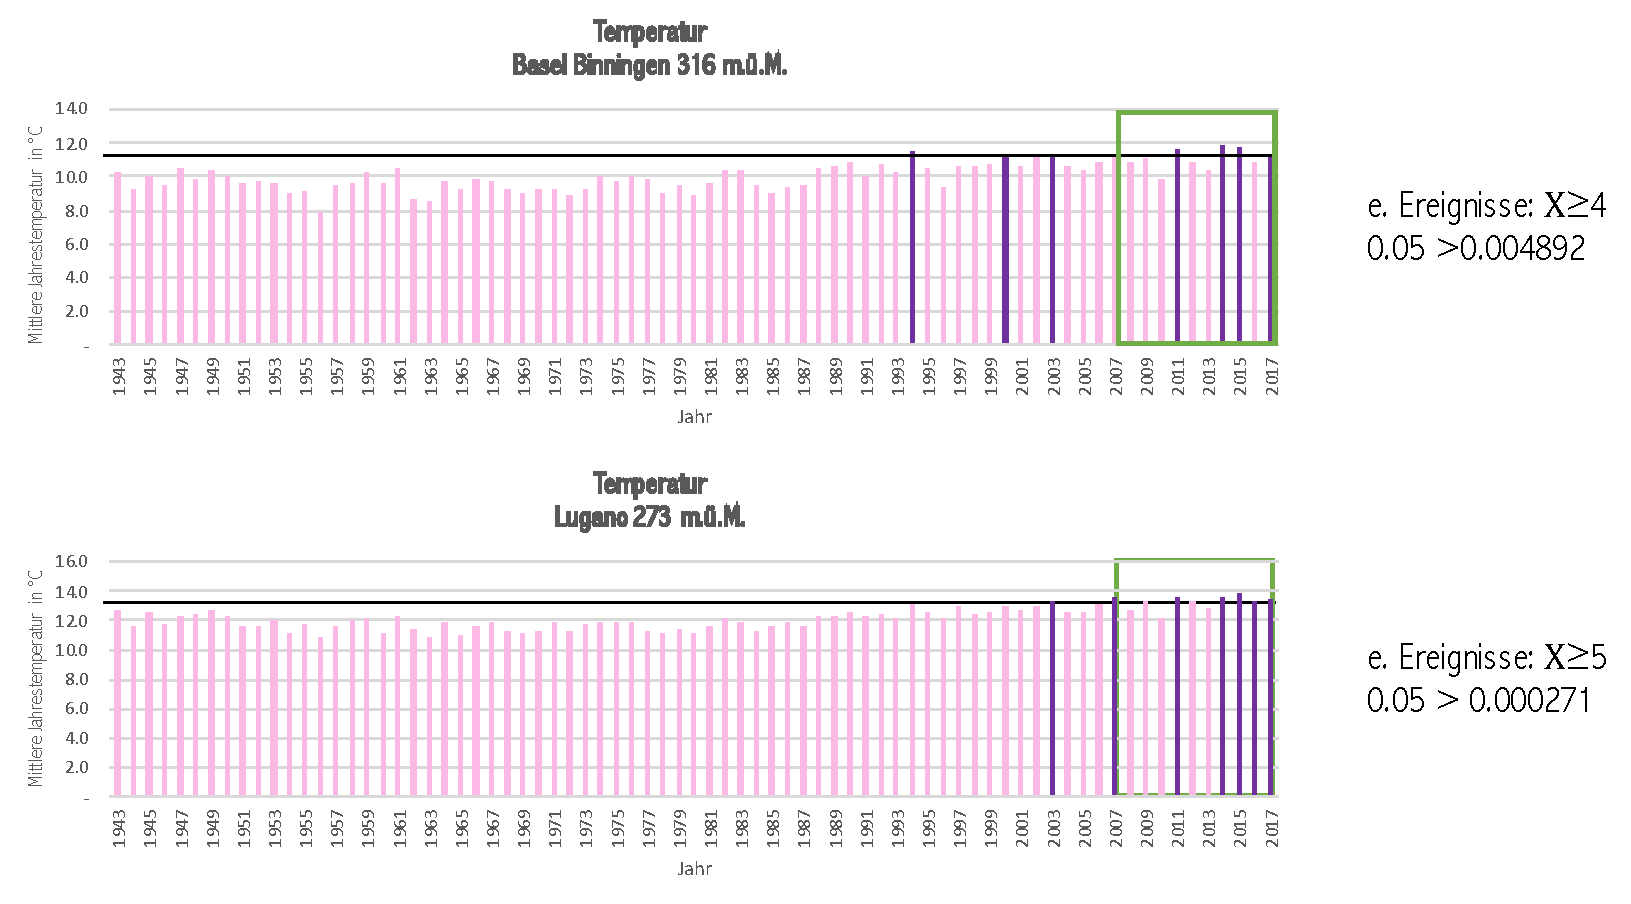
\includegraphics[width=1.0\textwidth]{extrem/JMittel.pdf}
\caption{BLaBLa}
\label{JMittel}
\end{figure}

\begin{figure}
\centering
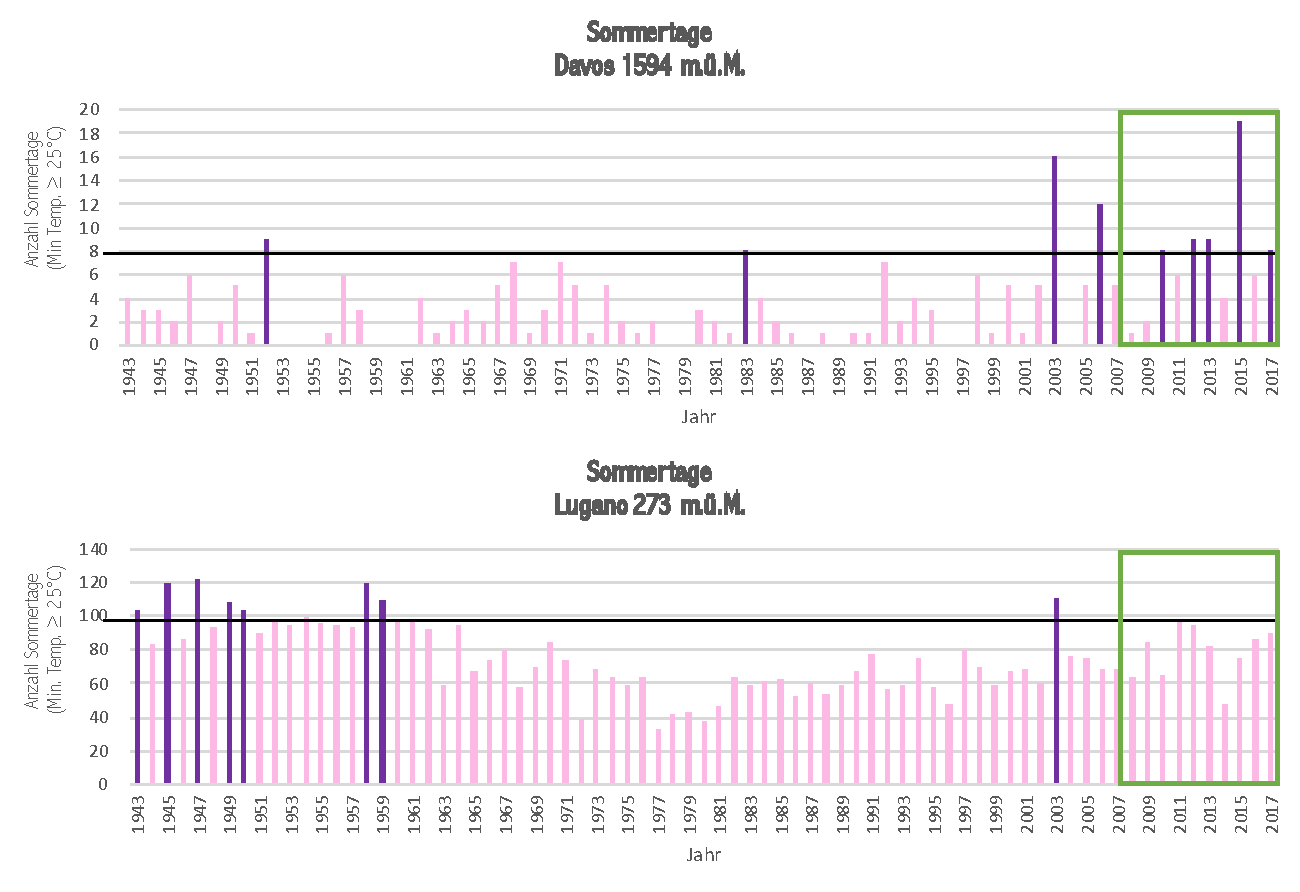
\includegraphics[width=1.0\textwidth]{extrem/Sommertage.pdf}
\caption{BLaBLa}
\label{Sommertage}
\end{figure}




\begin{figure}
\centering
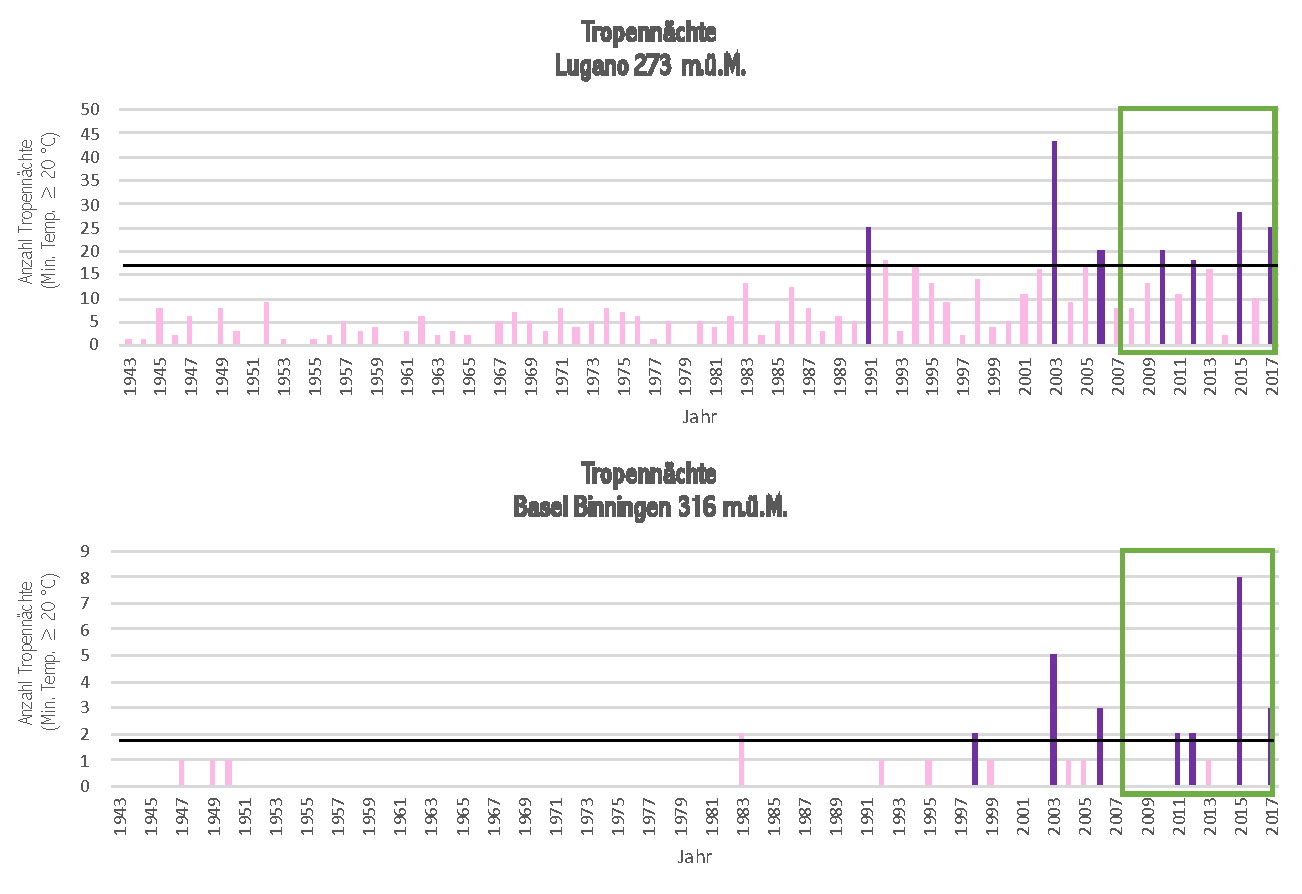
\includegraphics[width=1.0\textwidth]{extrem/Tropennacht.pdf}
\caption{BLaBLa}
\label{Tropennacht}
\end{figure}



\begin{figure}
\centering
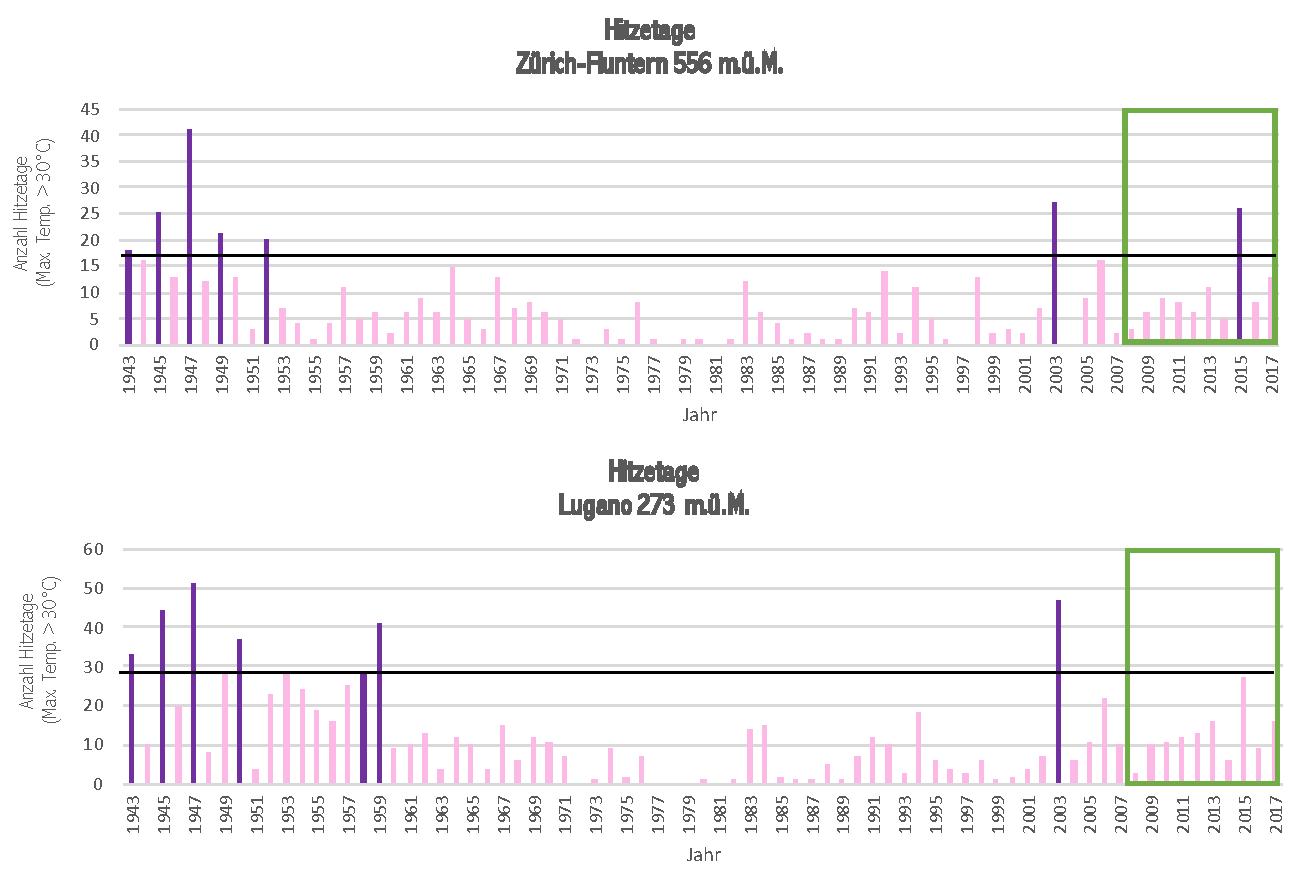
\includegraphics[width=1.0\textwidth]{extrem/Hitzetage.pdf}
\caption{BLaBLa}
\label{Hitzetage}
\end{figure}


\begin{figure}
\centering
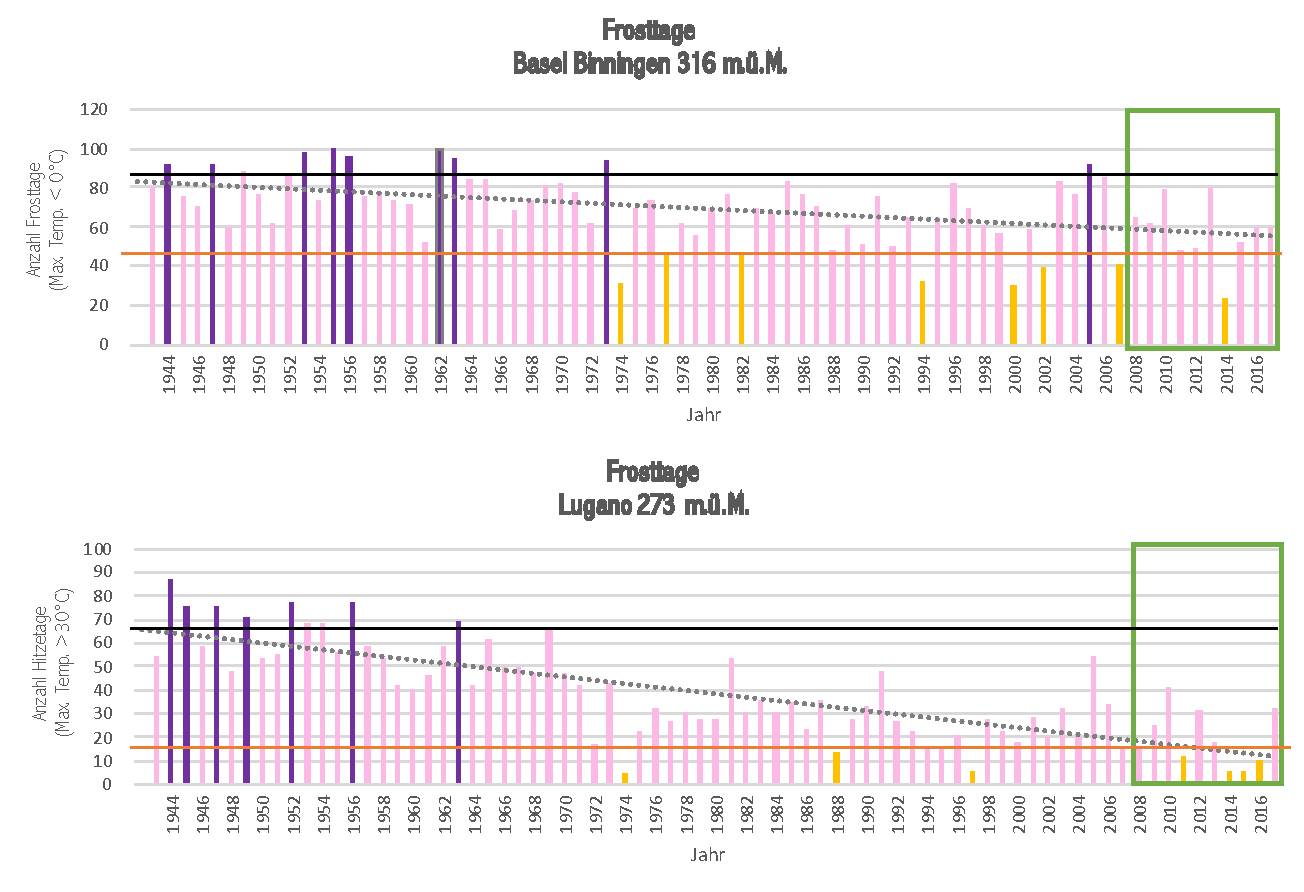
\includegraphics[width=1.0\textwidth]{extrem/Frosttage.pdf}
\caption{BLaBLa}
\label{Frosttage}
\end{figure}


\begin{figure}
\centering
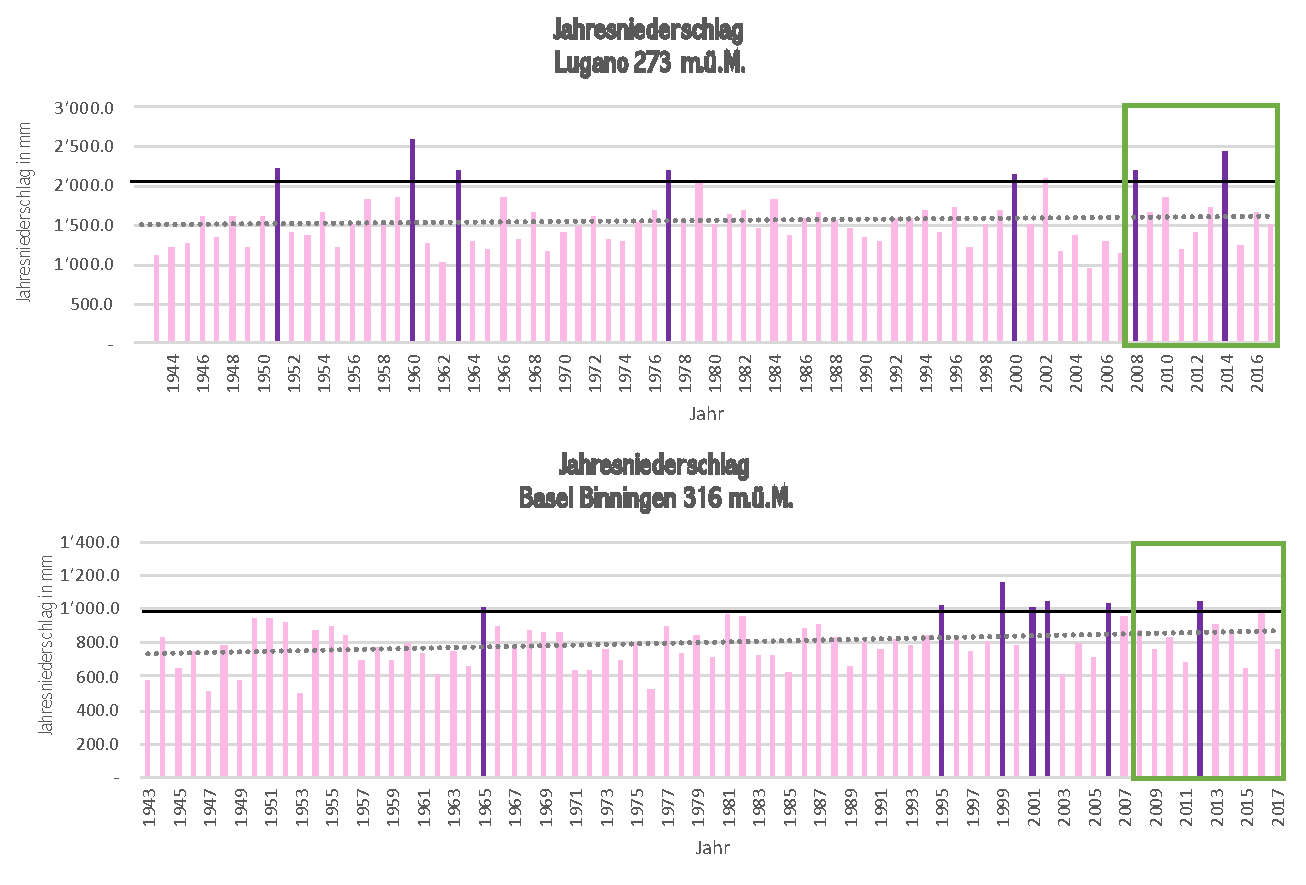
\includegraphics[width=1.0\textwidth]{extrem/Jahresniederschlag.pdf}
\caption{BLaBLa}
\label{Jahresniederschlag}
\end{figure}

\begin{figure}
\centering
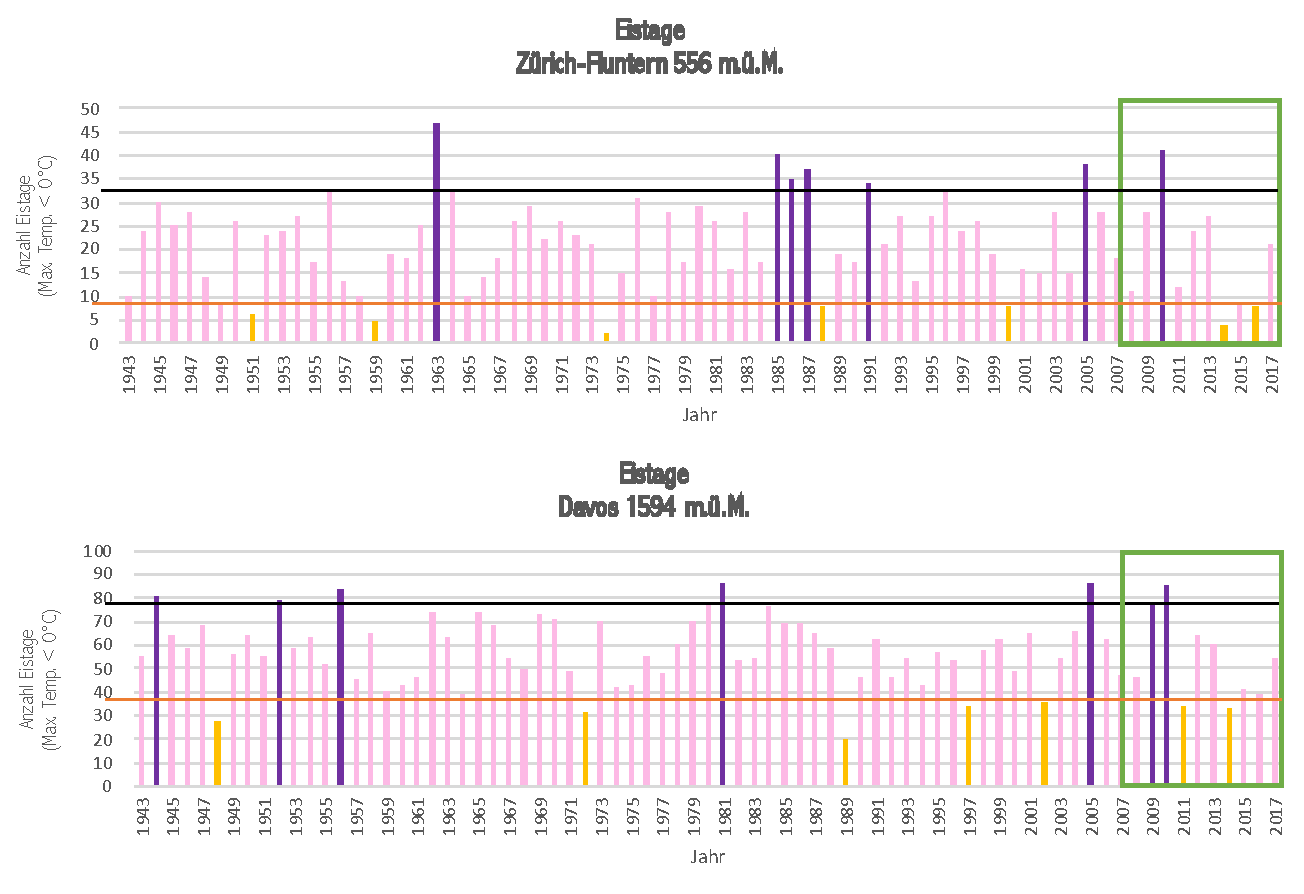
\includegraphics[width=1.0\textwidth]{extrem/Eistage.pdf}
\caption{BLaBLa}
\label{Eistage}
\end{figure}


\rhead{Schlussfolgerung}
Der Klimawandel ist real.

\rhead{Abschnitt}



\printbibliography[heading=subbibliography]
\end{refsection}
